\begin{savequote}[8cm]
  ``Those who can, do; those who can't, teach.''
  \qauthor{Dan Zevin}
\end{savequote}
\makeatletter
\chapter{Applications}
\label{Applications}

\section{Fast Summation}

A essential task in modern spherical approximation methods is the fast evaluation of linear combinations $f$ of (space localizing) spherical radial basis functions $K$,  
\begin{equation}
  \label{Applications:KernelSum}
  f: \twosphere \rightarrow \R,\ \fun{f}{\xi} := \sum_{l = 0}^{L-1} 
    b_{l} \fun{K}{\V{\eta}_{l} \cdot \V{\xi}} \quad \paren{\V{\xi} \in \twosphere}
\end{equation}
on a set of \emph{target nodes} 
$$
  \mathcal{X} := \pset{\V{\xi}_{d} \in \twosphere}{|}{d=0,\ldots,D-1,\ D \in \N}
$$ 
with 
$$
  \mathcal{Y} := \pset{\V{\eta}_{l} \in \twosphere}{|}{l = 0,\ldots,L-1,\ L \in \N}
$$
being the set of \emph{source nodes}, $b_{l} \in \R$ and $\fun{K}{\V{\eta} \: \cdot}$ a \emph{radial spherical basis function} or \emph{$\V{\eta}$-zonal function} 
\[
  \fun{K}{\V{\eta} \: \cdot}: \twosphere \rightarrow \R,\ \V{\xi} \mapsto \fun{K}{\V{\eta} \cdot \V{\xi}} \quad \paren{\V{\xi} \in \twosphere}.\]

The naive approach, i.e. evaluating \eqref{Applications:KernelSum} for every $\V{\xi}_{d} \in \mathcal{X}$ clearly leads to an $\bigo{L\:D}$ algorithm. For large $L$ and $D$ the computational effort becomes quickly unaffordable.
The \emph{panel clustering} method introduced in \cite{FrGlSch98} reduces the computational effort to evaluate \ref{Applications:KernelSum} based on the traditional method of dividing the evaluation into near- and far-field. For every kernel, the near-field contribution is calculated exactly whereas the contribution of the far-field may be approximated coarsly due to the rapid decay. 

The approach presented here is a a cutoff in frequency-domain. Using \eqref{Basics:Kernel}, we obtain
%$$
%  \fun{f}{\xi} = \sum_{l = 0}^{L-1} b_{l} \sum_{k=0}^{\infty} \beta_{k} \fun{P_k}{\V{\eta}_{l} \cdot \V{\xi}}.
%$$
%Now using the Addition Theorem \ref{} we can write
\[
  \fun{K}{\V{\eta}_{l} \cdot \V{\xi}} = \sum_{k=0}^{\infty} \sum_{n=-k}^k \fun{K^{\wedge}}{k} \fun{Y_{k}^n}{\V{\xi}} \overline{\fun{Y_{k}^n}{\V{\eta}_{l}}}
\]
and by truncating at a finite index $M \in \NZ$, i.e. defining
\[
  \fun{K_{M}}{\V{\eta}_{l} \cdot \V{\xi}} := 
  \sum_{k=0}^{M} \sum_{n=-k}^k \fun{K^{\wedge}}{k} \fun{Y_{k}^n}{\V{\xi}} \overline{\fun{Y_{k}^n}{\V{\eta}_{l}}}
\]
we obtain
\begin{equation}
  \begin{split}
    \fun{f}{\xi} \approx \fun{f_{M}}{\xi} & := \sum_{l = 0}^{L-1} b_{l} \fun{K_{M}}{\V{\eta}_{l} \cdot \V{\xi}} \\
                 &       = \sum_{l = 0}^{L-1} b_{l} \sum_{k=0}^{M} \sum_{n=-k}^k \fun{K^{\wedge}}{k}
                           \fun{Y_{k}^n}{\V{\xi}} \overline{\fun{Y_{k}^n}{\V{\eta}_{l}}} \\
                 &       = \sum_{k=0}^{M} \sum_{n=-k}^k \fun{K^{\wedge}}{k}
                           \fun{Y_{k}^n}{\V{\xi}} \paren{\sum_{l = 0}^{L-1} 
                           b_{l} \overline{\fun{Y_{k}^n}{\V{\eta}_{l}}}}.
  \end{split}                           
\end{equation}
Evaluating the sums
\begin{equation}
\label{Applications:AdjointNDSFT}
  \tilde{b}_{k}^n := \sum_{l = 0}^{L-1} b_{l} \overline{\fun{Y_{k}^n}{\V{\eta}_{l}}} \quad \paren{k = 0,\ldots,M; n = -k,\ldots,k}
\end{equation}
corresponds to an adjoint NDSFT and we arrive at
\[
  \fun{f_{M}}{\xi} \approx \sum_{k=0}^{M} \sum_{n=-k}^k \tilde{b}_{k}^n \fun{K^{\wedge}}{k}
                       \fun{Y_{k}^n}{\V{\xi}} = \sum_{k=0}^{M} \sum_{n=-k}^k a_{k}^n
                       \fun{Y_{k}^n}{\V{\xi}}
\]
with $a_{k}^n := \tilde{b}_{k}^n \fun{K^{\wedge}}{k}$. Finally, the evaluation of
\begin{equation}
\label{Applications:NDSFT}
  \sum_{k=0}^{M} \sum_{n=-k}^k a_{k}^n \fun{Y_{k}^n}{\V{\xi}_{d}} \quad \paren{\V{\xi}_{d} \in \mathcal{X}}
\end{equation}
is a NDSFT. In matrix-vector this reads
\[
  \fun{\V{f}}{\mathcal{X}} = \fun{\V{Y}}{\mathcal{X}} \: \V{W} \: \fun{\V{Y}}{\mathcal{Y}}^{\h} \: \V{b}
\]
with
\begin{align}
  \fun{\V{f}}{\mathcal{X}} & := \paren{\fun{f}{\V{\xi}_{d}}}_{d=0}^{D-1} \in \R^D,\\
  \fun{\V{Y}}{\mathcal{X}} & := \paren{\fun{Y_k^n}{\V{\xi}_{d}}}_{d=0,\ldots,D-1; \paren{k,n} \in \mathcal{I}^M} \in \C^{D \times \paren{M+1}^2}. \\
  \V{W} & := \fun{\diag}{\V{w}},\ \V{w} := \paren{w_{k}^n}_{\paren{k,n} \in \mathcal{I}^M} \in \R^{(M+1)^2},\ w_{k}^n := \fun{K^{\wedge}}{k}, \\
  \fun{\V{Y}}{\mathcal{Y}} & := \paren{\fun{Y_k^n}{\V{\eta}_{l}}}_{l=0,\ldots,L-1; \paren{k,n} \in \mathcal{I}^M} \in \C^{L \times \paren{M+1}^2}
\end{align}
The NDSFT \eqref{Applications:NDSFT} and the adjoint NDSFT in \eqref{Applications:AdjointNDSFT} can be computed by the fast NFSFT and adjoint NFSFT algorithms, i.e. Algorithm \ref{} and \ref{}, respectively. In total, we obtain an $\bigo{M^2 \log^2 M + mL + mD}$ algorithm summarized in Algorithm \ref{}
\begin{algorithm}[ht]
  \caption{Fast Summation}
  \label{Applications:Algorithm:FastSummation}    
  \begin{algorithmic}
    \STATE  Input:  $L \in \N$, $\paren{b_{l}}_{l=0}^{L-1}$, $\paren{\V{\eta}_{l}}_{l=0}^{L-1}$, 
                    $D \in \N$, $\paren{\V{\xi}_{d}}_{d=0}^{D-1}$, $M \in \NZ, \paren{\fun{K^{\wedge}}{k}}_{k=0}^M$
    \STATE
    \STATE Compute $\paren{\tilde{b}_{k}^n}_{\paren{k,n} \in \mathcal{I}^M}$ by a fast adjoint NFSFT
    \STATE 
    \FOR {$k=0,\ldots,M$} 
      \FOR {$n=-k,\ldots,k$} 
        \STATE $a_{k}^n := \tilde{b}_{k}^n \fun{K^{\wedge}}{k}$
      \ENDFOR
    \ENDFOR
    \STATE
    \STATE Compute $\paren{\fun{f}{\V{\xi}_{d}}}_{d=0}^{D-1}$ by a fast NFSFT
    \STATE
    \STATE Output: $\paren{\fun{f}{\V{\xi}_{d}}}_{d=0}^{D-1}$
\end{algorithmic}
\end{algorithm}
This approximation causes a pointwise truncation error 
\begin{eqnarray*}
  \fun{K_{\text{\textsl{err}}}}{\V{\eta}_{l} \cdot \V{\xi}} 
    & := & \abs{\fun{K}{\V{\eta}_{l} \cdot \V{\xi}} - \fun{K_{M}}{\V{\eta}_{l} \cdot \V{\xi}}}\\
    &  = & \abs{\sum_{k=M+1}^{\infty} \sum_{n=-k}^k \fun{K^{\wedge}}{k} \fun{Y_{k}^n}{\V{\eta}_{l}} \overline{\fun{Y_{k}^n}{\V{\xi}}}}.
\end{eqnarray*}
Using \eqref{Basics:OrthogonalKernelExpansion} and the fact that $\max_{x \in \interv{[}{-1}{1}{]}} \abs{\fun{P_{k}}{x}} = 1$, we have
\[
  \fun{K_{\text{\textsl{err}}}}{\V{\eta}_{l} \cdot \V{\xi}} 
  = \abs{\sum_{k = M+1}^{\infty} \frac{2k+1}{4\pi} \fun{K^{\wedge}}{k} \fun{P_k}{\V{\eta}_{l} \cdot \V{\xi}}} 
  \le \sum_{k = M+1}^{\infty} \abs{\frac{2k+1}{4\pi} \fun{K^{\wedge}}{k}} =: \fun{\varepsilon}{M}.
\]
If the coefficients $b_{l}$ in \eqref{Applications:KernelSum} are assumed to be comparable, then the pointwise error $\fun{f_{\text{\textsl{err}}}}{\xi}$ in $\fun{f}{\V{\xi}}$ can be estimated by
\[
  \fun{f_{\text{\textsl{err}}}}{\xi} := \abs{\fun{f}{\xi} - \fun{f_{M}}{\xi}} 
  \le \sum_{l=0}^{L-1} b_{l} \fun{K_{\text{\textsl{err}}}}{\V{\eta}_{l} \cdot \V{\xi}}
  \le \sum_{l=0}^{L-1} b_{l} \fun{\varepsilon}{M}
  \le C L \fun{\varepsilon}{M}
\]
for some constant $C \in \Rp$.
\begin{example}
  We applied Algorithm 
\end{example}

\section{Iterative Fourier Reconstruction}

\begin{figure}[tb]
  \centering
  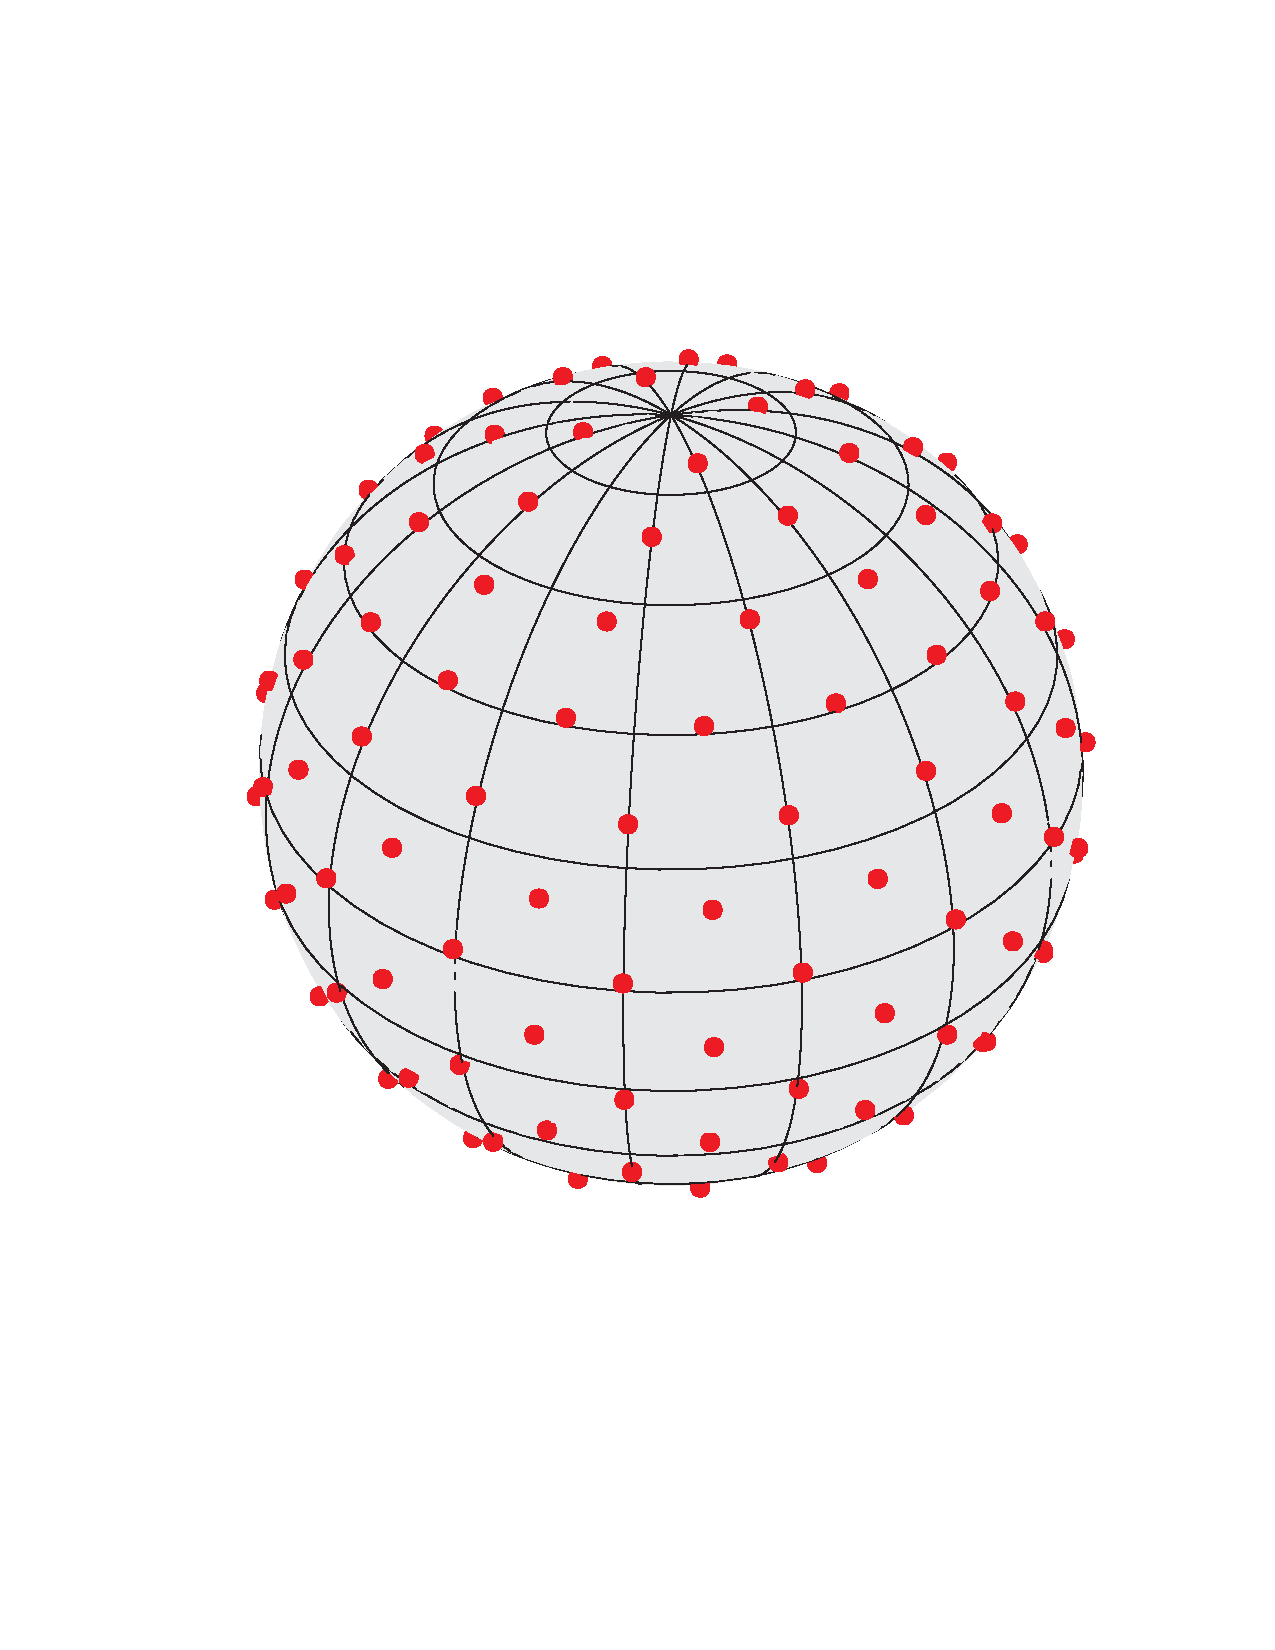
\includegraphics[width=12cm]{images/healpix}
  \caption{To be written...}
  \label{healpix}
\end{figure}


